\chapter{Bevezetés}

A konzulensem, Dr. Szegletes Luca már régóta gyűjt videokártyás kódimplementációkat különböző NP-nehéz problémákra. Amikor megbeszéltük, hogy mi lenne a dolgom, különböző útkeresési algoritmusok megvalósítását kaptam feladatul. A jármű útvonaltervezési algoritmusoknak nagyon sok alesete van, ugyanis végtelenül sokféle feltételeket szabhatunk meg egy bejárás számára: a teljes hossz legyen rövid, az egyes utak legyenek egyenként rövidek, stb. Különböző alkalmazásokhoz nagyon változatos elvárások dukálnak: például ha egy bútor szállítmányozási cég akarja kitalálni, hogy az aznapi 20 klienséhez milyen sorrendben juttassa el az árukat, már azt is bele kell kalkulálnia, hogy hogyan fognak a termékek beleférni egy kamionba (véges kapacitás problémája). Másik példa egy nemzetközi körutazás: a cég vezérigazgatója be szeretné járni egy kampány keretében a cég különböző leányvállalatait, melyek a mai világ bármely pontján lehetnek: lehet, hogy az egyik üzem Kolumbia közepén, míg egy másik valahol Indiában van. A két ország időzónája nagyon különböző, ezért nem mindegy, hogy az igazgató a nap melyik órájában szeretné magát fogadtatni a helyi vezetőkkel (a kliens nem korlátlanul áll rendelkezésre, igazítani kell a fogadó és vendég beosztását). Még számtalan hasonló szituáció képzelhető el, ezek, amiket említettem csak a legtipikusabbak. Ezen problémákat a számítástudomány már évtizedek óta számon tartja, hátha lehet előrébb jutni velük. 

\begin{figure}[ht!]
	\centering
	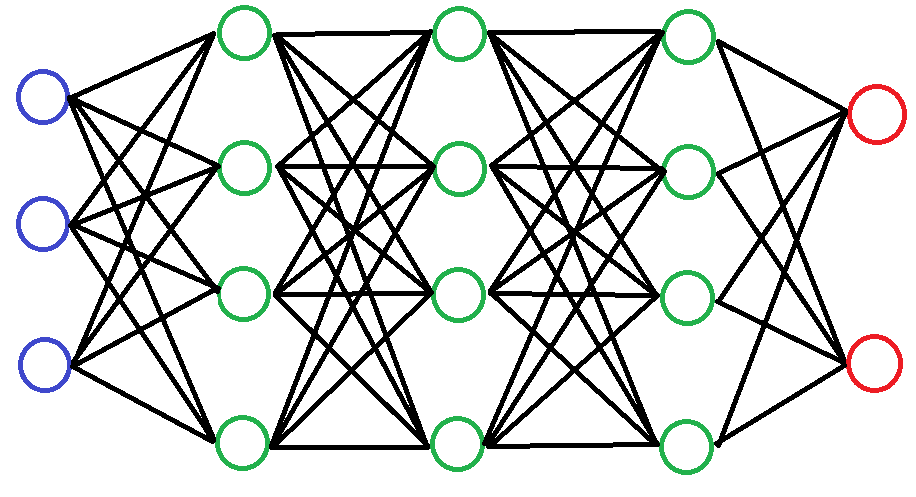
\includegraphics[width=150mm, keepaspectratio]{figures/neurons.png}
	\caption{Többféle modellt is kitaláltak már gépi tanuláshoz, az egyik leghíresebb az ún. neuronháló modell }
\end{figure}
A mai világban a mesterséges intelligencia forradalmasította a számítástechnikát a számítási kapacitások soha eddig nem látott bővülése miatt. Az NVIDIA egy olyan cég ,mely hardvergyártóként, konkrétan videokártyák gyártásával és értékesítésével kezdte. Az elmúlt években komoly szerkezetváltozáson megy keresztül, igyekszik némileg közönséget is váltani: korábban a videokártyák legnagyobb felvevőpiaca a videojátékosok voltak. A GPU arra lett kitalálva, hogy különböző 2D-, 3D-s renderelési feladatokban tehermentesítse a CPU-t. Több (fizikai) ezer szálon képes futni. Egy GPU szál cserébe sokkal szűkebb utasításkészleten tud dolgozni, mint egy CPU szál. A GPU szálak elsősorban különböző aritmetikai utasítások végrehajtásában jeleskednek: rendelkeznek hardveres FPU-val (floating point unit - olyan hardver, mely lebegőpontos számokon végzett aritmetikára lett tervezve). 
A mesterséges intelligenciát használó algoritmusok azért lettek forradalmi vívmányok, mert az algoritmus kiötletelésének nehézségeit nagyrészt képes kivenni a programozók kezéből. Egy klasszikus program írása során a kódírónak teljes körű elképzelése kell legyen arról, hogy hogyan fog eljutni az eredményhez. 



\begin{figure}[ht!]
	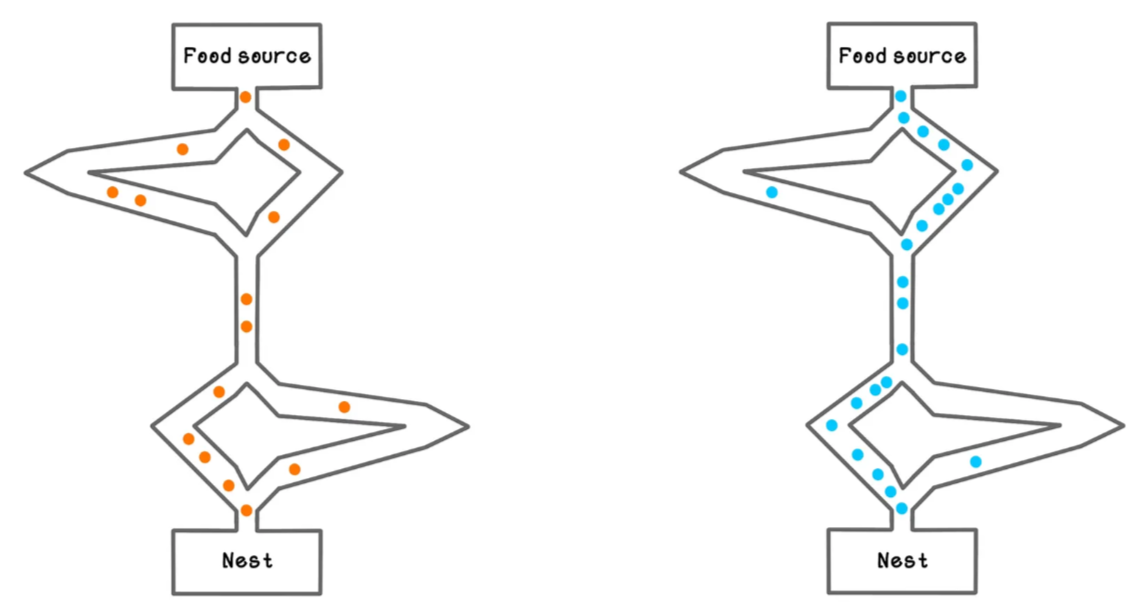
\includegraphics[width=150mm, keepaspectratio]{figures/aco-visualization.png}
	\caption{A hangyák sajátos módon optimalizálják a táplálékszerzést: a Hangyakolónia Optimalizáció segítségével \cite{ACOimage} \label{ACOvisulabel}}
\end{figure}
A gépi tanulás másképp működik: az én esetemben, a \textbf{genetikus algoritmusoknál} kell hozzá egy input, és egy hibafüggvény. A programozó megadja, hogy mely bemenetre szeretné ráengedni az algoritmust. Az algoritmus kap még egy kiértékelő függvényt, amellyel számszerű eredményt rendelhet az általa alkotott megoldásokhoz. A épnek van memóriaterülete, amelyet az alapján írhat, hogy mit tanult. A genetikus algoritmusok megoldásgenerációkat hoznak létre. A gép a hibafüggvény segítségével értékeli az egyes genomokat, majd a legjobban sikerült egyedek alapján készít következő generációt. A folyamat többféle módon is véget érhet:
\begin{itemize}
	\item a hibafüggvény egy adott hibahatáron belüli megoldást talál
	\item at algoritmus adott ideig (pl. 2 óra) fut, a végő megoldás az utolsó generáció legjobb megoldása
	\item a program adott számú iterációt hajt végre, a végső megoldást készítheti külön, a korábban tanultak alapján
\end{itemize}

A gép kiveszi a programozó kezéből az algoritmizálási feladatot. A kódoló választ egy modellt, amely alapján a gép majd dolgozik. Ha elégedetlenek vagyunk, választhatunk másik modellt, hátha az sikeresebbnek bizonyul.

Szakdolgozatom során a \textbf{Hangyakolónia optimalizáció} modelljét alkalmaztam. Ez egy természetből ellesett trükkön alapuló gráfbejárási algoritmus, a hangyák élelemkeresési módszereire hasonlít. Szemléleti a \ref{ACOvisulabel}. ábra



A hangyák egész nap a hangyaboly környékét járják morzsák, elhullott rovarok után kutatva. Amikor egy dolgozó korábban felfedezetlen élelemforrást talál, kis részével visszaindul a bolyba, és a hazaúton egyfajta testnedvet, \textbf{feromon}t bocsát ki magából. A többi hangya megérzi a szagot, és a nyomába megy. Ha tényleg táplálékhoz vezetett a feromoncsík, akkor ők is kis részével visszaindulnak az élőhelyükre. A folyamat egészen addig tart, amíg van mit elvinni. Ezután az utólag érkező hangyák azt tapasztalják, hogy elfogyott, ezért ők visszafelé már nem eresztenek anyagot. A szél előbb-utóbb elfújja az úton hagyott feromont, ezért nem megy oda több hangya.

\section{Fejezetek}
A rövid bevezetés után először ismertetem a problémák elméleti hátterét. Matematikailag kimondom a feladatokat, valamint bemutatom, milyen - főleg valószínűségszámítási - alapok szükségesek a Hangyakolónia optimalizáció alapos megértéséhez.



